\begin{figure}[htbp]
    \centering
    \includegraphics[scale=1]{figure/grating.png}
    \caption{回折格子における光の回折}
\end{figure}
% https://dl.cdn-anritsu.com/ja-jp/test-measurement/files/Technical-Notes/White-Paper/MS9740A_JR1100.pdf

\begin{figure}[htbp]
    \centering
    \includegraphics[scale=1]{figure/achromaticlense.png}
    \caption{アクロマティックレンズでの色収差の補正}
\end{figure}
% http://www.mekatoro.net/digianaecatalog/chuo-sougou/book/chuo-sougou-P0904.pdf


\begin{figure}[htbp]
    \centering
    \includegraphics[scale=0.8]{figure/spectrometer_design.png}
    \caption{分光器概略図}
\end{figure}


\floatsetup[figure]{style=plain,subcapbesideposition=top}
\begin{figure}
    \sidesubfloat[]{
        \includegraphics[scale=0.7]{figure/lense_system.png}}
    \sidesubfloat[]{
        \includegraphics[scale=0.7]{figure/grating_system.png}}
    \caption{.
    (a):レンズ周りの部品構成
    (b):回折格子周りの部品構成}
\end{figure}

\floatsetup[figure]{style=plain,subcapbesideposition=top}
\begin{figure}
    \sidesubfloat[]{
        \includegraphics[scale=0.5]{figure/HeNe_focus_before.png}}
    \sidesubfloat[]{
        \includegraphics[scale=0.5]{figure/HeNe_focus_after.png}}
    \caption{HeNeレーザを光源にした際の$\pm{1}$次光のスペクトル幅とフォーカスパルスの関係性
    (a):平面鏡$m_3$の位置はそのままでスリット台は10mmのものを使用して撮影
    (b):平面鏡$m_3$の位置を6.5mm前にしスリット台は30mmのものを使用して撮影}
\end{figure}


\floatsetup[figure]{style=plain,subcapbesideposition=top}
\begin{figure}
    \sidesubfloat[]{
        \includegraphics[scale=0.5]{figure/meikou_before.png}}
    \sidesubfloat[]{
        \includegraphics[scale=0.5]{figure/meikou_after.png}}
    \caption{スリットに光を入れないで撮影した際の強度分布.露光時間は1秒,x軸方向,y軸方向ともにビニングサイズを4とした.
    (a):分光器内に壁を取り付ける前に撮影したもの
    (b):分光器内に壁を取り付けた後に撮影したもの}
\end{figure}


\begin{figure}[htbp]
    \centering
    \includegraphics[scale=1]{figure/lambda-grating_fitting.png}
    \caption{波長と回折格子パルスの対応図}
\end{figure}


\floatsetup[figure]{style=plain,subcapbesideposition=top}
\begin{figure}
    \sidesubfloat[]{
        \includegraphics[scale=0.5]{figure/lambda-focus_fitting_1st.png}}
    \sidesubfloat[]{
        \includegraphics[scale=0.5]{figure/lambda-focus_fitting_-1st.png}}
    \caption{波長とフォーカスパルスの対応図\\
    (a):1次光のフィッテイング結果
    (b):-1次光のフィッテイング結果}
\end{figure}

\begin{figure}[htbp]
    \centering
    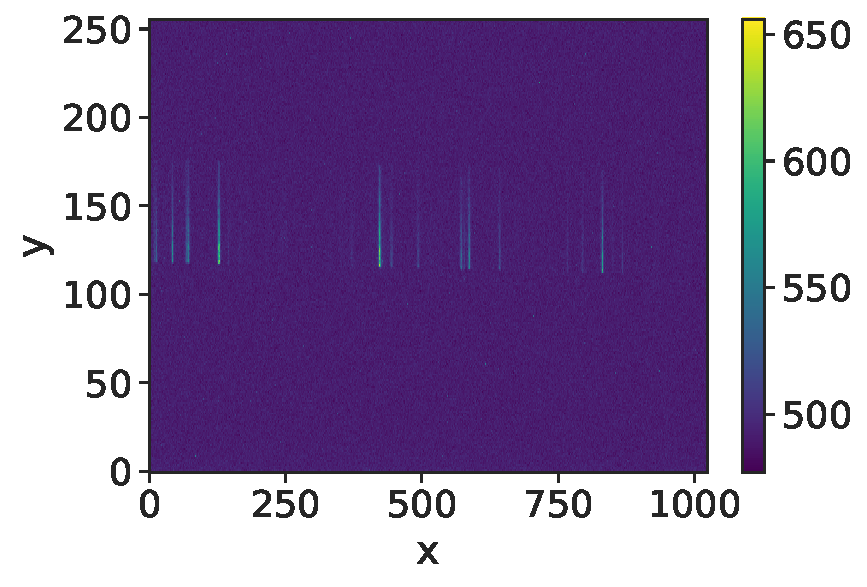
\includegraphics[scale=1]{figure/spectrum_example.png}
    \caption{光源をFeランプで撮影した波長520nm付近の光の二次元強度分布}
\end{figure}

\begin{figure}[htbp]
    \centering
    \includegraphics[scale=1]{figure/spectrum_example2.png}
    \caption{光源をFeランプで撮影した波長520nm付近のスペクトル}
\end{figure}

\begin{figure}[htbp]
    \centering
    \includegraphics[scale=0.5]{figure/fe_wide_range.png}
    \caption{光源をFeランプで撮影した測定波長範囲でのスペクトル}
\end{figure}


